\documentclass[12pt,hyperref={pdfpagelabels=false},notes=show,aspectratio=169]{beamer}

\usetheme[]{FFF}

% Bugfix for pdfpagelables=false
\providecommand\thispdfpagelabel[1]{}

% Standard packages

\usepackage[english,ngerman]{babel}
\usepackage[utf8]{inputenc}
\usepackage{times}

% Setup TikZ

\usepackage{tikz}
\usetikzlibrary{arrows}
\tikzstyle{block}=[draw opacity=0.7,line width=1.4cm]

% Text \us
\usepackage{textcomp}
\usepackage{mathcomp}

% Textpos
\usepackage[absolute,overlay]{textpos}
\setlength{\TPHorizModule}{\paperwidth}
\setlength{\TPVertModule}{\paperheight}

% Blitz-Symbol
\usepackage{stmaryrd}

% Tabellen
\usepackage{multirow}
\usepackage{array}
\usepackage{colortbl}
\definecolor{lightblue}{rgb}{ 0.55, 0.55, 1.00}
\definecolor{lightred}{rgb}{  1.00, 0.35, 0.35}
\definecolor{lightgreen}{rgb}{0.50, 1.00, 0.50}
\newcommand{\ccg}{\cellcolor{lightgreen}}
\newcommand{\ccr}{\cellcolor{lightred}}
\newcommand{\ccb}{\cellcolor{lightblue}}

% Listings
\usepackage{listings}

\setlength{\parindent}{0cm}

% Stroke
\usepackage{ulem}

% vc
\input{vc.tex}

%%%%%%%%%%%%%%%%%%%%%% /LAYOUT %%%%%%%%%%%%%%%%%%%%%%%%%%%%


% Author, Title, etc.

\title{Freifunk Franken und das V2 Debakel}

\subtitle{Freifunk Festival 2018}

\author[Tim Niemeyer]{Tim Niemeyer {\tiny \textless{}tim@tn-x.org\textgreater{}}\texorpdfstring{\tiny \\
                        7E7B~3401~42AA~9295~B8F2~~~6C4C~20A9~F38D~2945~ECB5\\\\
                        https://github.com/RedDog99/vortrag-erlug2018.git~~~~\VCRevisionMod}{}}

\date[06.10.2018]{6.10.2018}

\newcommand{\zb}{z.\,B.\@}
\newcommand{\us}{~\textmu{}s}
\newcommand{\uv}{~\textmu{}V}
\newcommand{\ms}{~ms}

\begin{document}

\usebackgroundtemplate{
\includegraphics[height=\paperheight,width=\paperwidth]{slides_background_title}}

\beamertemplatenavigationsymbolsempty
\begin{frame}[plain,squeeze]
	\maketitle
\end{frame}\addtocounter{framenumber}{-1}

\usebackgroundtemplate{
\includegraphics[height=\paperheight,width=\paperwidth]{slides_background}}

\begin{frame}{Inhalt}
    \hspace{0.1\textwidth}
    \parbox[c][0.8\textheight][s]{0.8\textwidth}{
        \tableofcontents
    }
\end{frame}

%%%%%%%%%%%%%%%%%%%%%% CONTENT %%%%%%%%%%%%%%%%%%%%%%%%%%%%

\section{Freifunk}

\begin{frame}{Einleitung}
    \begin{itemize}
        \item Freifunk Franken ist lokaler Ableger der Freifunk-Bewegung (freifunk.net)
        \item Nicht-kommerzielle Initiative für freie Funknetzwerke\\
        \begin{itemize}
            \item[$\rightarrow$] Bürger investieren in Eigenregie Zeit, Geld und Enthusiasmus
        \end{itemize}
        \item Nicht nur \glqq{}kostenloses Internet\grqq $\Rightarrow$ \glqq{}freies Netzwerken\grqq\\
        \begin{itemize}
            \item Lokal intressante Dienste zur Verfügung stellen (Webcams)
            \item Text, Musik und Filme über das interne Freifunk-Netz übertragen
            \item Über lokale Dienste Chatten oder Telefonieren
        \end{itemize}
    \end{itemize}
\end{frame}

\begin{frame}{Wie es funktioniert}
    \begin{itemize}
        \item Freifunker stellen WLAN-Router für sich selbst und den Datentransfer der anderen Teilnehmer zur Verfügung
        \begin{itemize}
            \item ggf. mit Anschluss an das www (für VPN)
        \end{itemize}
        \item Benachbarte Router verbinden sich und spannen ein sogenanntes Mesh-Netzwerk auf
        \item Nicht benachbarte Router verbinden sich mittels VPN-Tunnel zum Freifunk
        \item Jegliche Verbindung ins www wird hierüber umgeleitet, um Risiken der Störerhaftung zu entgehen
    \end{itemize}
\end{frame}

\begin{frame}{Was braucht man?}
    \begin{itemize}
        \item Ein günstiger, unterstützter Router (ab ca. 17€)
        \item Eine spezielle Firmware
        \item Die Zustimmung zum \glqq{}Pico-Peering Agreement\grqq
        \begin{itemize}
            \item Regelwerk, das grundsätzliche Eigenschaften eines Freifunk-Netzwerkes sichert
            \begin{enumerate}
                \item Freier Transit
                \item Offene Kommunikation
                \item Keine Garantie (Haftungsausschluss)
                \item Nutzungsbestimmungen
                \item Lokale (individuelle) Zusätze
            \end{enumerate}
            \item Die Freifunk Firmware implementiert diese Grundsätze standardmäßig
        \end{itemize}
    \end{itemize}
\end{frame}


\section{Grundlagen}
\begin{frame}{}
    \begin{center}
        Grundlagen
     \end{center}
\end{frame}

\begin{frame}{Ein typisches Freifunk Netz}
    \begin{itemize}
        \item Ein Batman-Adv Netz
        \begin{itemize}
            \item[$\rightarrow$] "Wie ein großer dezentraler Switch"
        \end{itemize}
        \item VPN für die Funkinseln
        \begin{itemize}
            \item Multi-Client zu Multi-Client VPN
            \item Layer-II Netz
            \item Kein internes Routing / Forwarding
        \end{itemize}
        \item Mehrere VPN Server / Gateway
        \begin{itemize}
            \item DHCP
            \item DNS Namensauflösung
            \item Gateway zum Internet / ICVPN
        \end{itemize}
        \item Monitoring
        \begin{itemize}
            \item Karte aller Knoten
        \end{itemize}
    \end{itemize}
\end{frame}

\begin{frame}{Ein typisches Freifunk Netz}
    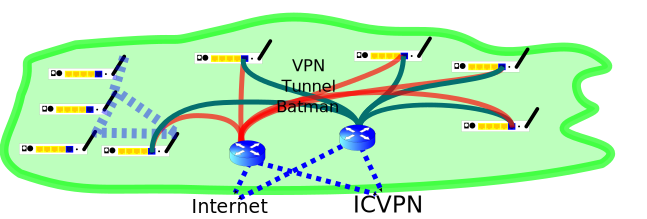
\includegraphics[width=\textwidth]{img/svg/freifunk_konzepte_alt.pdf}
\end{frame}

\begin{frame}{Freifunk Franken Netz}
    \includegraphics[width=\textwidth]{img/svg/freifunk_konzepte.pdf}

    \begin{itemize}
        \item Mehrere Layer-2 Inseln (Hoods)
        \item Verbindung per Layer-3
        \item Dezentrale Gateways
    \end{itemize}
\end{frame}

\begin{frame}{Knoten VPN}
    \begin{itemize}
        \item Verwendetes VPN: fastd
        \begin{itemize}
            \item n:m VPN
        \end{itemize}
        \item Endpunkt Vermittlung über KeyXchange:
        \begin{itemize}
            \item Zentrale Webseite \only<2-3>{{\color{red}Problem!}}
            \item Knoten meldet sich mit Standort
            \item Geographisch nächste Hood wird zugewiesen (voronoi)
            \item Client bekommt Liste aller Server der Hood
        \end{itemize}
        \item<3> Keine weitere Unterscheidung zu welcher Hood der Knoten gehört
        \item<3> {\color{red}Problem!} Funk Verbindung zwischen den Hoods
    \end{itemize}
\end{frame}

\begin{frame}{VPN Server}
    \begin{itemize}
        \item VPN Server: In jeder Hood gibt es mehrere davon
        \item Hoodzuweisung manuell im KeyXchange
        \item DHCP
        \begin{itemize}
            \item Aktuell ausschließlich IPv4
            \item Unterschiedliche Latenzen: Ungleiche Server Auslastung
            \begin{itemize}
                \item[$\rightarrow$] Batman-Adv GW Selection
                \item Anpassung nach Traffic Auslastung
            \end{itemize}
        \end{itemize}
        \item DNS Namesauflösung
        \item Policy base routing
        \item VPN (GRE) Tunnel zu anderen Gateways
        \begin{itemize}
            \item OLSR Routing
        \end{itemize}
    \end{itemize}
\end{frame}

\begin{frame}{Gateways}
    \begin{itemize}
        \item Verbindet Freifunk und Internet
        \item IPv4 NAT (oft übers Ausland) ins Internet
        \item Announced 0.0.0.0/0 via OLSR
        \begin{itemize}
            \item Dynamic Gateway Plugin
            \item VPN Server können diese Routen nutzen
        \end{itemize}
        \item Routing Metrik ohne Traffic/Bandbreite
        \item<2> {\color{red}Problem!} Ungleiche Traffic Verteilung
    \end{itemize}
\end{frame}

\section{Freifunk V2}

\begin{frame}{}
    \begin{center}
        Freifunk V2
     \end{center}
\end{frame}

\begin{frame}{Die Idee}
    Neuer keyXchange ...

    \begin{itemize}
        \item Knoten schickt Standort
        \item KeyXchange stellt Hood-File (passend zum Standort) bereit
        \item Knoten konfiguriert
        \begin{itemize}
            \item VPN
            \item WLAN
            \item IPv6 Netz
        \end{itemize}
        \item[$\rightarrow$] Unbeabsichtigte Hood-Verbindungen werden vermieden
    \end{itemize}
\end{frame}

\begin{frame}{Hood-File}
    \begin{itemize}
        \item Version
        \item ULA Prefix
        \item VPN Zugang: Protokoll, IP, Port, Key
        \item Hood-Daten: 
        \begin{itemize}
            \item Name, AP-ESSID
            \item BSSID, MESH\_ID, MESH\_ESSID
            \item Mesh-Protokoll (Batman-Adv)
            \item 2.4 und 5 GHz Kanal, Bandbreite, Mesh\_Type
            \item Upgrade URL, Zeit-Server
            \item Zeit-Stempel
            \item Standort der Hood
        \end{itemize}
    \end{itemize}
\end{frame}

\begin{frame}{Freifunk V2}
    \center
    \only<1>{Klingt ja eigentlich ganz gut}
    \only<2>{... aber}
\end{frame}

\begin{frame}{Der Uplink Knoten}
    \begin{itemize}
        \item keyXchange erreichbar
        \item Download Hood-File
        \item Konfigurieren
        \item Fertig.. Prima..
    \end{itemize}
\end{frame}

\begin{frame}{Mesh Knoten mit WLAN}
    \begin{itemize}
        \item Kein WAN: kein keyXchange erreichbar
        \item Keine Nachbarn (Knoten kennt die WLAN/Mesh Config nicht)
        \item Woher Hood-File nehmen?
        \item Suchen?
        \item[$\rightarrow$] Config-AP
    \end{itemize}
\end{frame}

\begin{frame}{Config-AP}
    \begin{itemize}
        \item Zusätzlicher (hidden) AP am Knoten
        \item Kleiner Webserver
        \item Stellt Hood-File zum Download bereit
        \item Mesh Knoten mit WLAN können Hood-File downloaden
    \end{itemize}
\end{frame}

\begin{frame}{Mesh Knoten mit Ethernet}
    \begin{itemize}
        \item Kein WAN: kein keyXchange erreichbar
        \item Batman-Adv läuft ja schon, Prima...
        \item WLAN-Settings? Woher nehmen?
        \item[$\rightarrow$] Hood-File vom Gateway laden
        \item[:(] Uplink-Knoten ändert sich
        \item[:(] Gateway und Uplink-Knoten sind unterschiedlich
        \item[:(] Es gibt mehrere Nachbarn: $\rightarrow$ Hood verbunden..
        \item[:(] Mesh Knoten bekommt Uplink: $\rightarrow$ ggfs Hood verbunden
    \end{itemize}
\end{frame}

\begin{frame}{Konstellationen}
    \begin{itemize}
        \item Knoten per Ethernet an Knoten per Ethernet an Uplink Knoten
        \item Knoten per Ethernet an Knoten per WLAN an Uplink Knoten
        \item Knoten per WLAN an Knoten per Ethernet an Uplink Knoten
        \item Knoten per WLAN an Knoten per WLAN an Uplink Knoten
        \item Mehrere Uplink Knoten
        \item Knoten per Ethernet und WLAN an Uplink
        \item Knoten mit 5 GHz und 2.4 GHz
        \item ... viele mehr ...
    \end{itemize}
\end{frame}

\begin{frame}{Sector-File}
    \begin{itemize}
        \item Ein Sector-File kann WLAN-Mesh Parameter überschreiben:
        \begin{itemize}
            \item WLAN Kanal
            \item Typ
            \item Mesh-ID
            \item AP-ESSID
        \end{itemize}
        \item Sector-File wird über Config-AP verteilt
        \begin{itemize}
            \item[:(] Nicht auf Ethernet
            \item[$\rightarrow$] Noch mehr Konstellationen
        \end{itemize}
    \end{itemize}
    \vfill
    \raggedleft
    \only<2>{... Ich erspare euch das weitere}
\end{frame}

\section{F3 Netze e.V.}

\begin{frame}{}
    \begin{center}
        F3 Netze e.V.
     \end{center}
\end{frame}

\begin{frame}{Verein ?}
    \begin{columns}[T]
        \begin{column}{0.45\textwidth}
            Was ist F3 Netze e.V.
            \begin{itemize}
                \item Infrastrukturverein
                \item IP-Ressourcen
                \item Provider $\rightarrow$ Traffic ''ausleiten''
                \item Standortüberlassungen
                \item Teilnehmer vom Freifunk Netz
                \item \underline{Keine} Community vertretung
            \end{itemize}
        \end{column}
        \begin{column}{0.45\textwidth}
            Was tut F3 Netze e.V.
            \begin{itemize}
                \item Freifunk Gateways
                \item Richtfunk-Standorte
                \item Tor Exit
                \item BFWA Frequenzen
            \end{itemize}
        \end{column}
    \end{columns}
\end{frame}

\begin{frame}{St. Paul}
    \center
    \only<1>{
        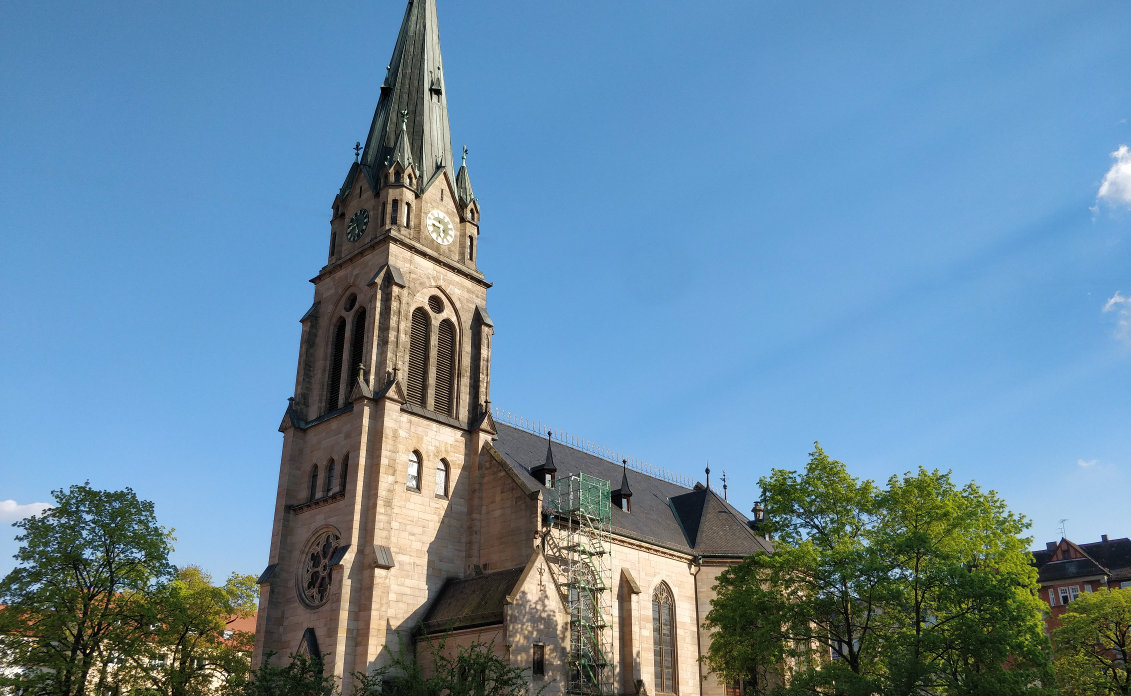
\includegraphics[height=0.86\textheight]{img/stpaul-turm}
    }
    \only<2>{
        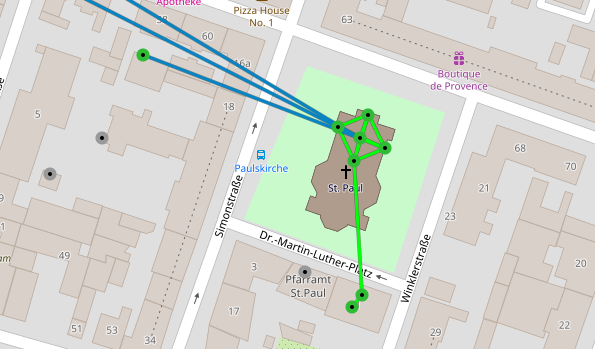
\includegraphics[height=0.86\textheight]{img/stpaul-karte}
    }
    \only<3>{
        \includegraphics[width=0.96\textwidth]{img/dia/stpaul}
    }
    \only<4>{
        ~
        \hfill
        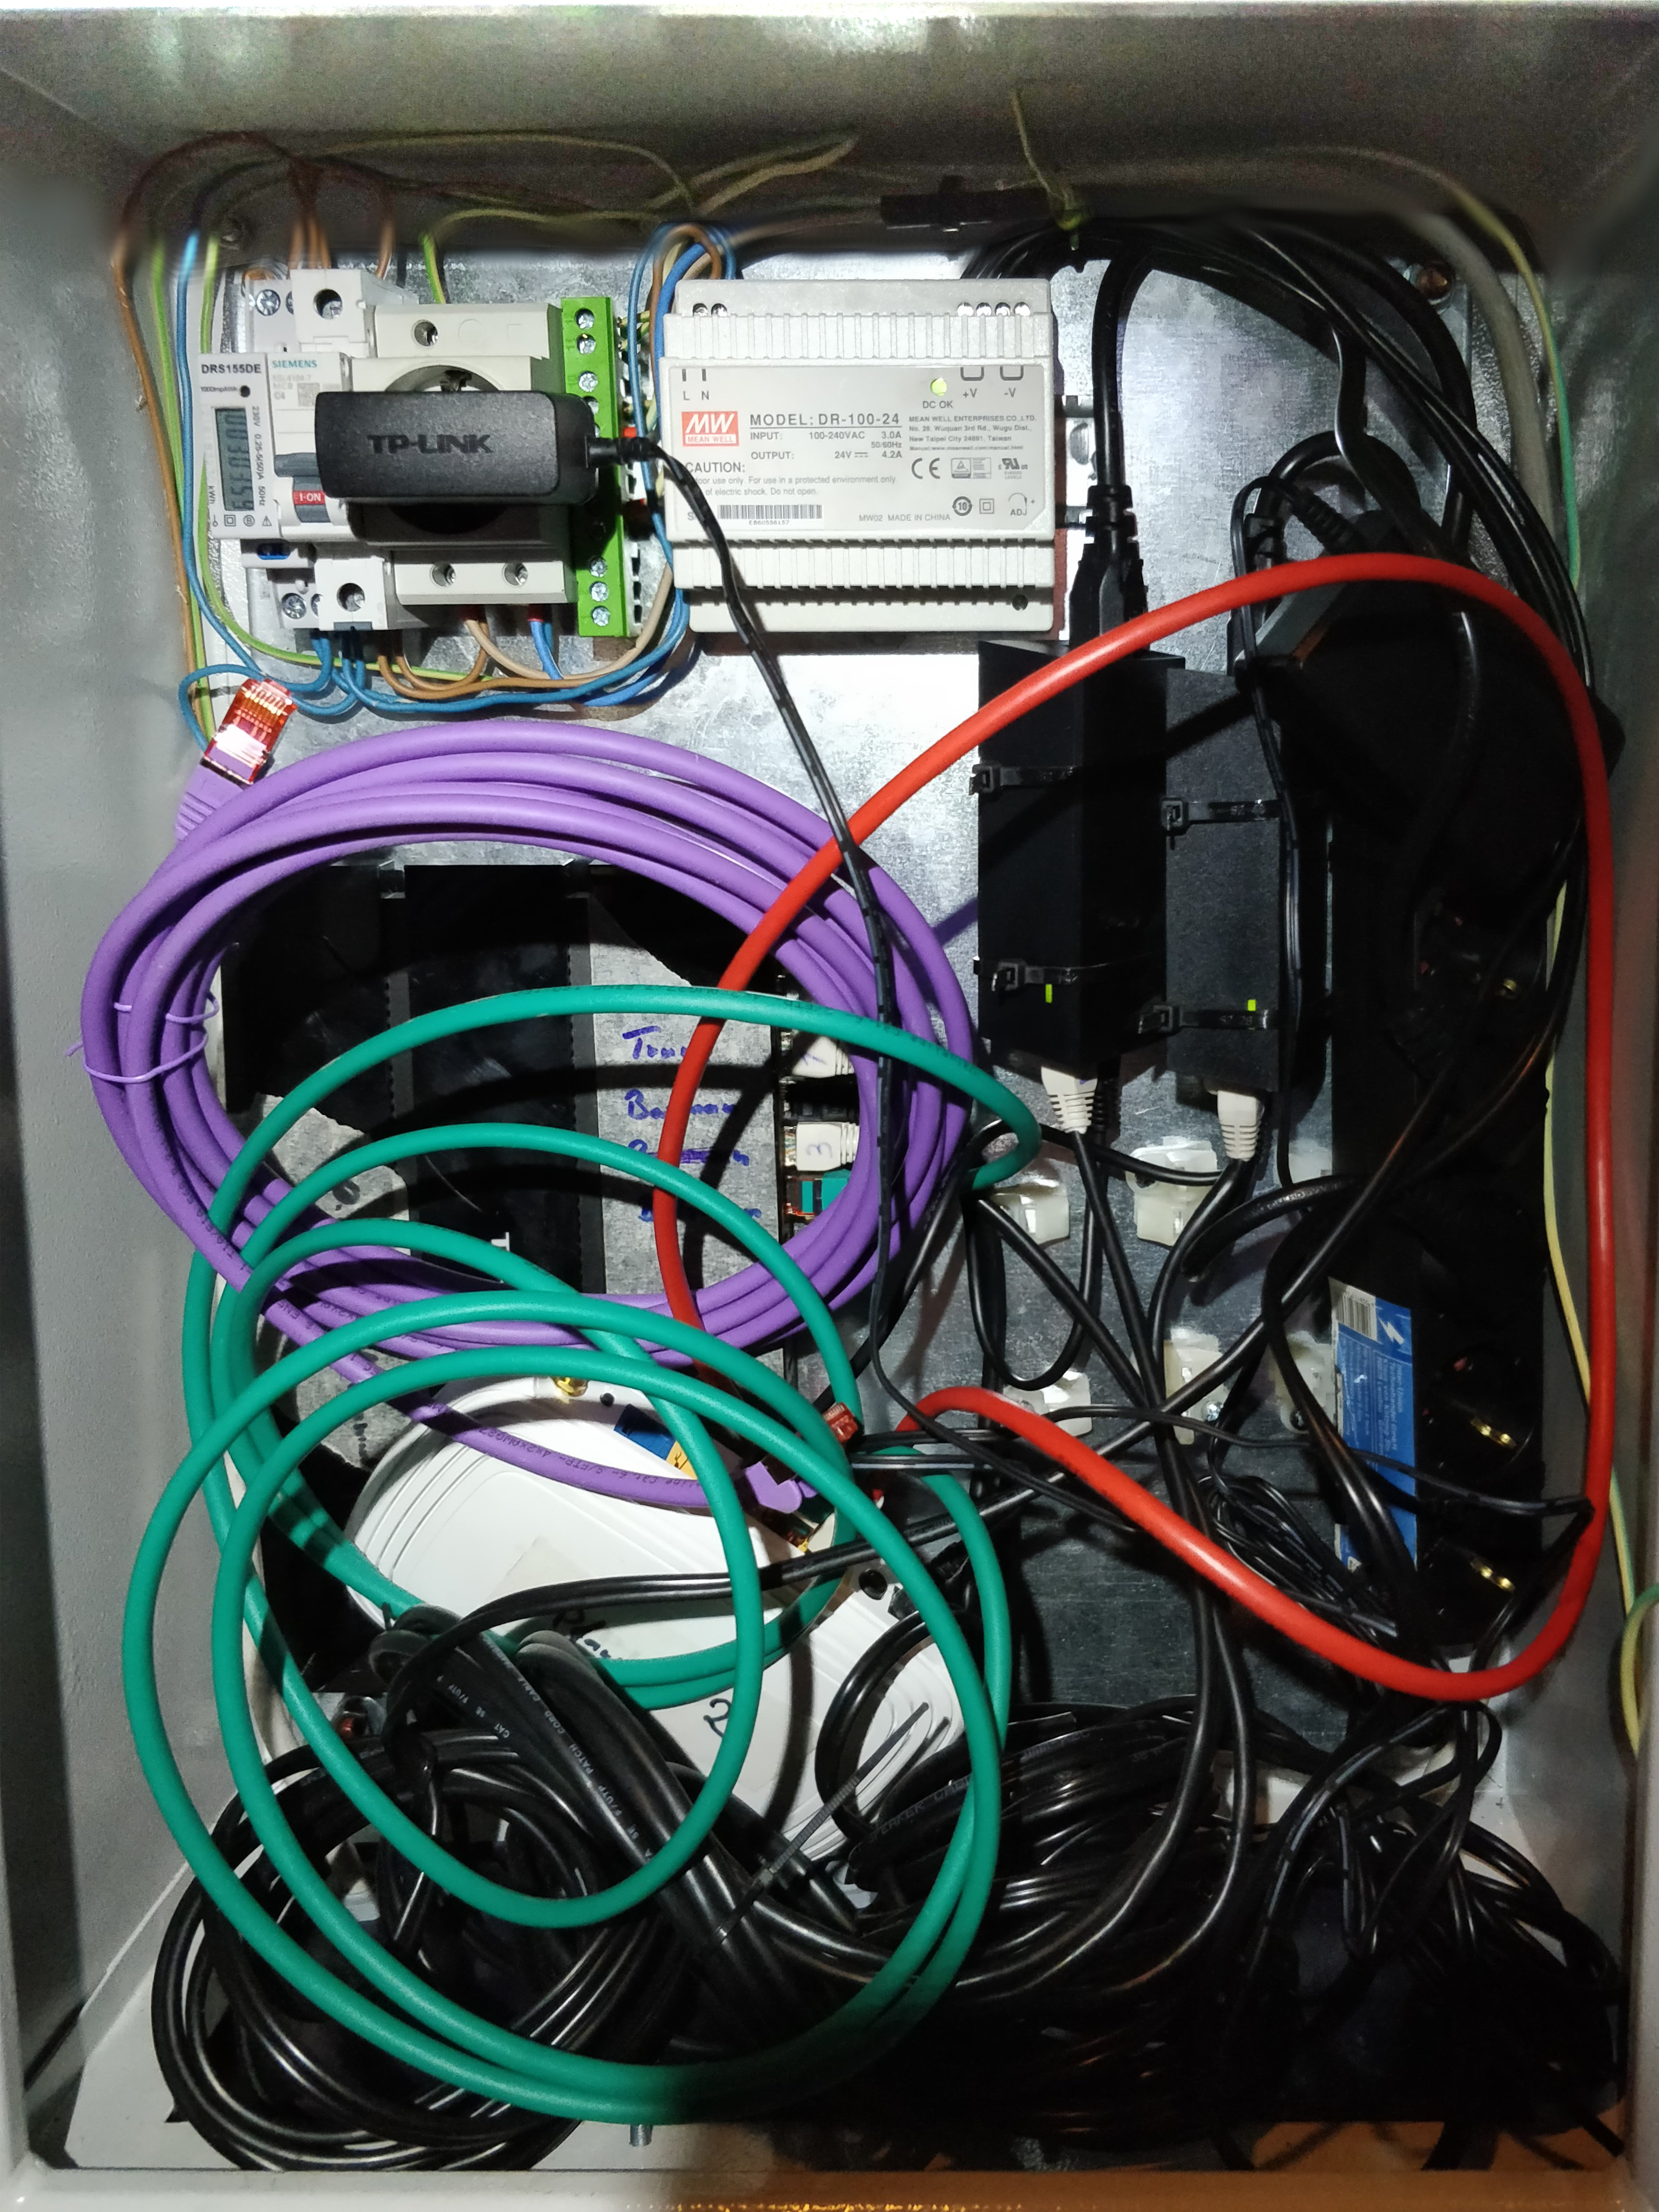
\includegraphics[height=0.86\textheight]{img/stpaul-kasten}
        \hfill
        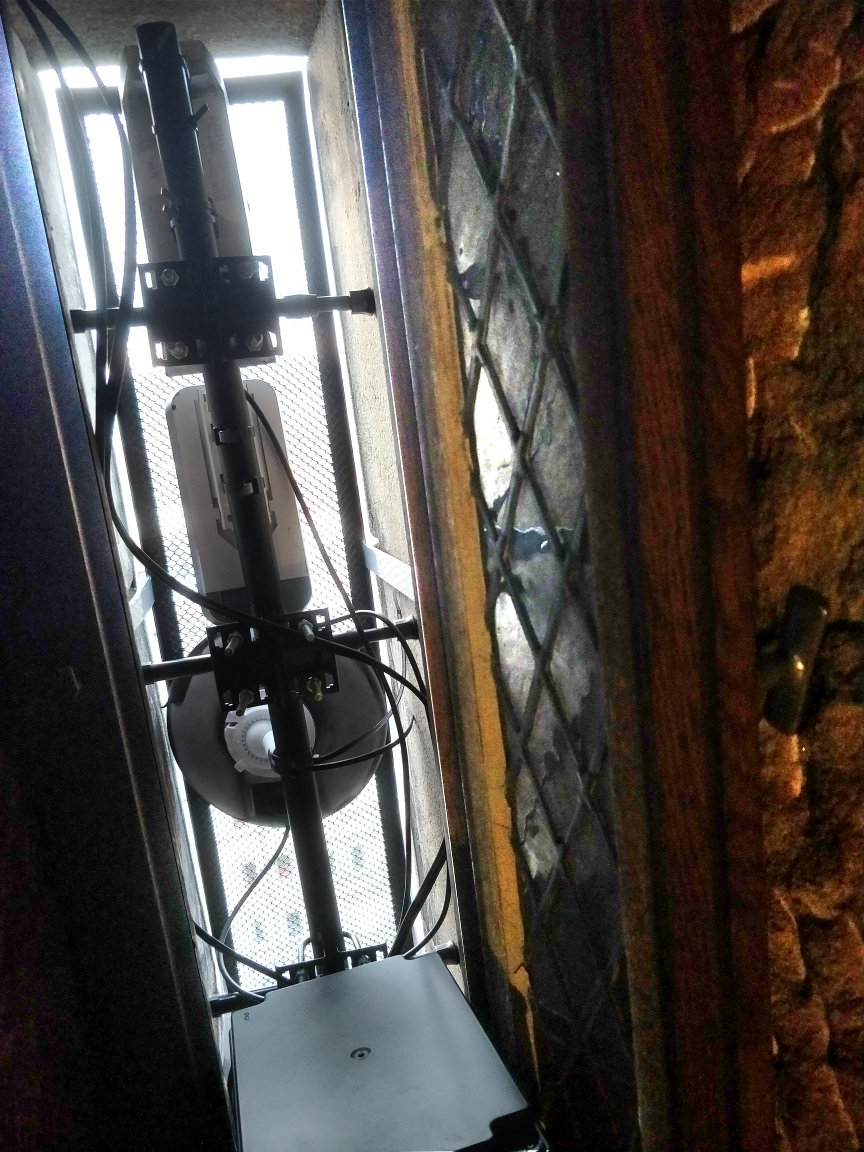
\includegraphics[height=0.86\textheight]{img/stpaul-fenster}
        \hfill
        ~
    }
\end{frame}

\begin{frame}{Z-Bau}
    \only<1>{
        \begin{itemize}
            \item IP-Ressourcen von den Zwiebelfreunde e.V.
            \begin{itemize}
                \item AS205100
                \item 185.220.100.0/24
                \item 2a0b:f4c0::/32
            \end{itemize}
            \item Glasfaser zum Nürnberg Internet Exchange (N-IX)
            \item 10 GBit/s Port von 
\includegraphics[height=1em]{img/proact}
            \item 800 MBit/s Transit
            \item $\sim$38 Peerings
            \item[$\rightarrow$] Aktuell ~400 MBit/s Tor Exit Traffic
        \end{itemize}
    }
    \only<2>{
        \center
        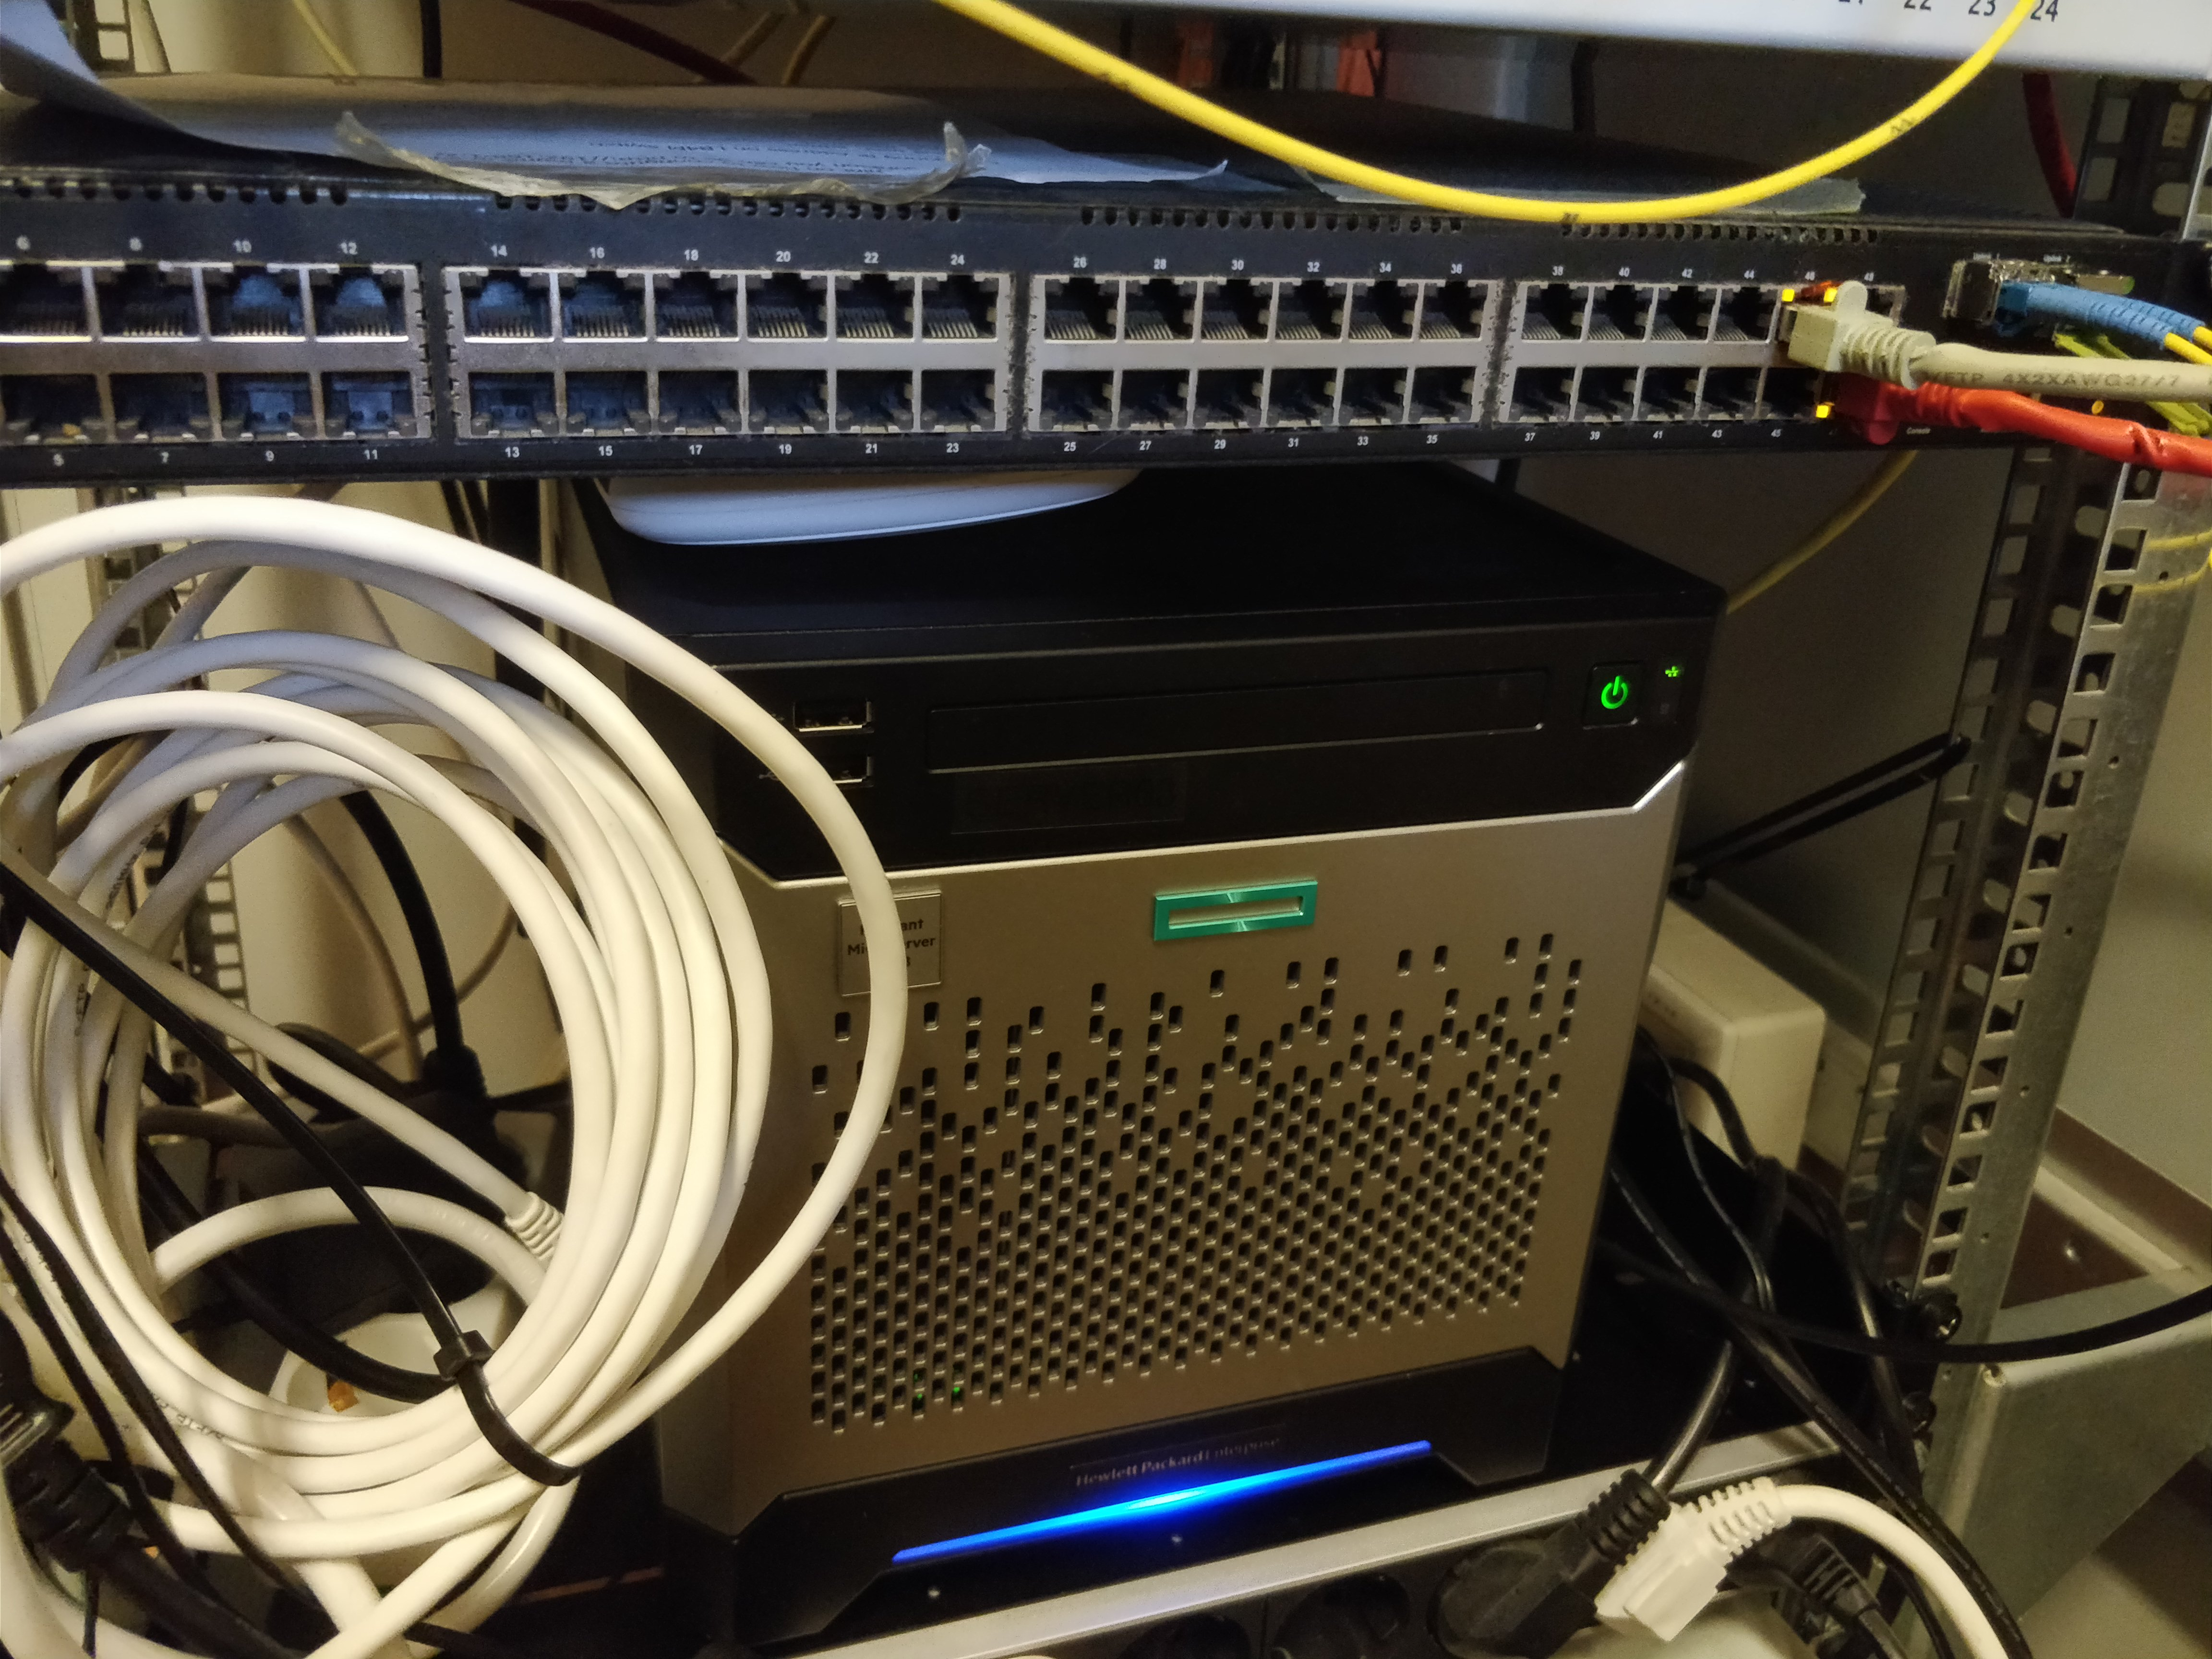
\includegraphics[height=0.86\textheight]{img/zbau-server}
    }
    \only<3>{
        \center
        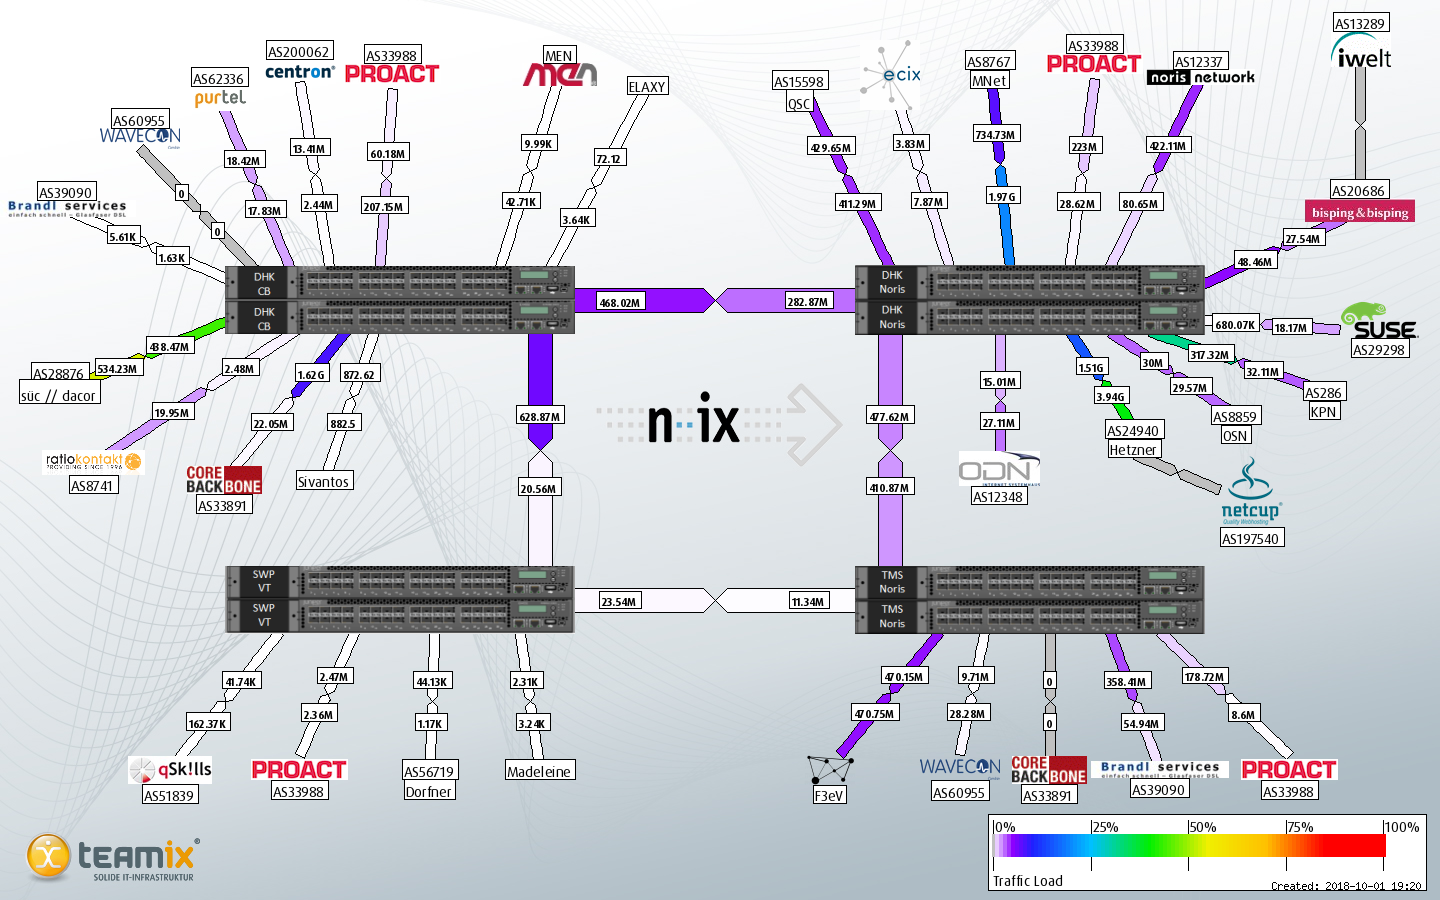
\includegraphics[height=0.86\textheight]{img/NIX}
    }
\end{frame}

\begin{frame}{Gemeinnützigkeit}
    \begin{columns}[T]
        \begin{column}{0.6\textwidth}
            \begin{itemize}
                \item Gemeinnützigkeit noch nicht anerkannt
                \item Verfahren pausiert
                \item Laut AEAO Liste aus §52 Absatz 2 Satz 1
                \item Laut AEAO ''Internetvereine'' per se nicht gemeinnützig
            \end{itemize}
        \end{column}
        \begin{column}{0.35\textwidth}
            
\includegraphics[width=\textwidth]{img/betterplace}
        \end{column}
    \end{columns}

    \vfill

    $\rightarrow$ Help needed\\
    \url{https://www.betterplace.org/de/projects/60168}

    \vfill
\end{frame}


\section{Freifunk V3}

\begin{frame}{}
    \begin{center}
        Freifunk V3
     \end{center}
\end{frame}

\begin{frame}{Warum?}
    \begin{itemize}
        \item \glqq{}Sofa-Knoten\grqq{} verstopfen das Netz, bringen wenig
        \item Wenig Know-How bei Knoten-Aufsteller
        \item Freifunk $\neq$ gratis Hotspot
        \item Mehr Zusammenarbeit
        \begin{itemize}
            \item[$\rightarrow$] Weniger \glqq{}Sofa-Knoten\grqq{}
            \item[$\rightarrow$] Mehr gegenseitige Vernetzung
        \end{itemize}
    \end{itemize}
\end{frame}

\begin{frame}{Die Idee}
    \begin{itemize}
        \item \only<1>{Neuer keyXchange}
            \only<2>{Nein, quatsch! ;)}
            \only<3>{Kein keyXchange mehr}
        \item<3> Es gibt keine spezielle Freifunk Firmware mehr
        \item<3> Kein automatisches Peering mehr
        \item<3> Dezentrale Gateways
        \item<3> \glqq{}Mesh Wolken\grqq{} mit fertigen Komponenten
    \end{itemize}
\end{frame}

\begin{frame}{Wie?}
    \begin{columns}[T]
        \begin{column}{0.46\textwidth}
            \begin{itemize}
                \item Back to the roots
                \item Nur ein Router mit
                \begin{itemize}
                    \item IP Subnetz(en): DHCP, Radvd, etc
                    \item Routing-Protokoll
                    \item VPN Software
                \end{itemize}
                \item Peerings von Hand über
                \begin{itemize}
                    \item Richtfunk
                    \item VPN
                    \item etc
                \end{itemize}
            \end{itemize}
        \end{column}
        \begin{column}{0.46\textwidth}
            \begin{itemize}
                \item Zugänge über
                \begin{itemize}
                    \item Kabel-Netzwerk
                    \item Access-Points
                \end{itemize}
                \item Kein Batman-adv
                \begin{itemize}
                    \item Google Wifi
                    \item AVM Mesh
                    \item TP-Link Deco
                    \item Ubnt UniFi Mesh
                    \item ... \url{http://lmgtfy.com/?q=wlan+mesh+loesungen}
                \end{itemize}
            \end{itemize}
        \end{column}
    \end{columns}
\end{frame}

\begin{frame}{St. Paul}
    \center
    \only<1>{
        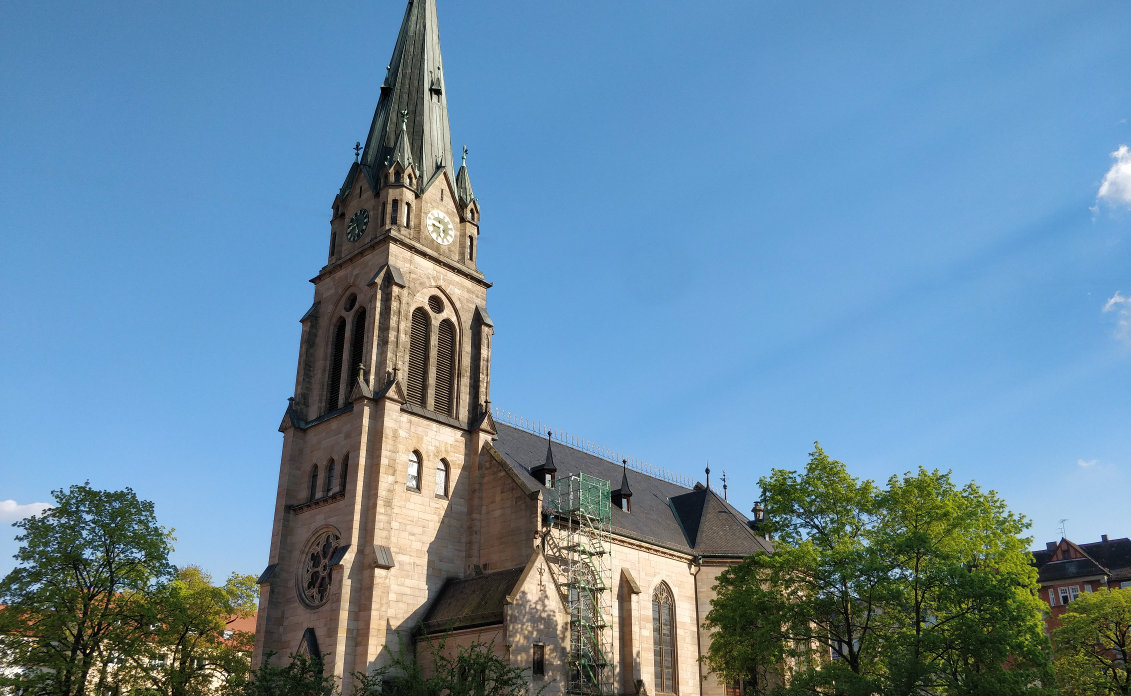
\includegraphics[height=0.86\textheight]{img/stpaul-turm}
    }
    \only<2>{
        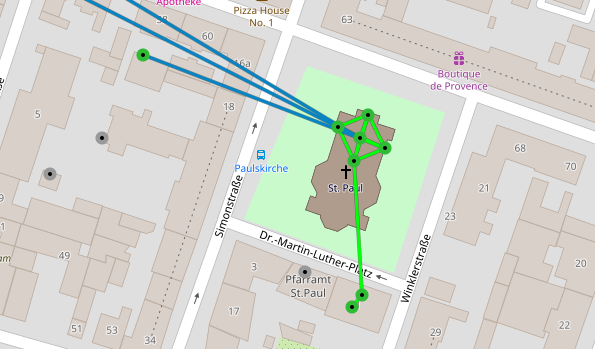
\includegraphics[height=0.86\textheight]{img/stpaul-karte}
    }
    \only<3>{
        \includegraphics[width=0.96\textwidth]{img/dia/stpaul}
    }
    \only<4>{
        ~
        \hfill
        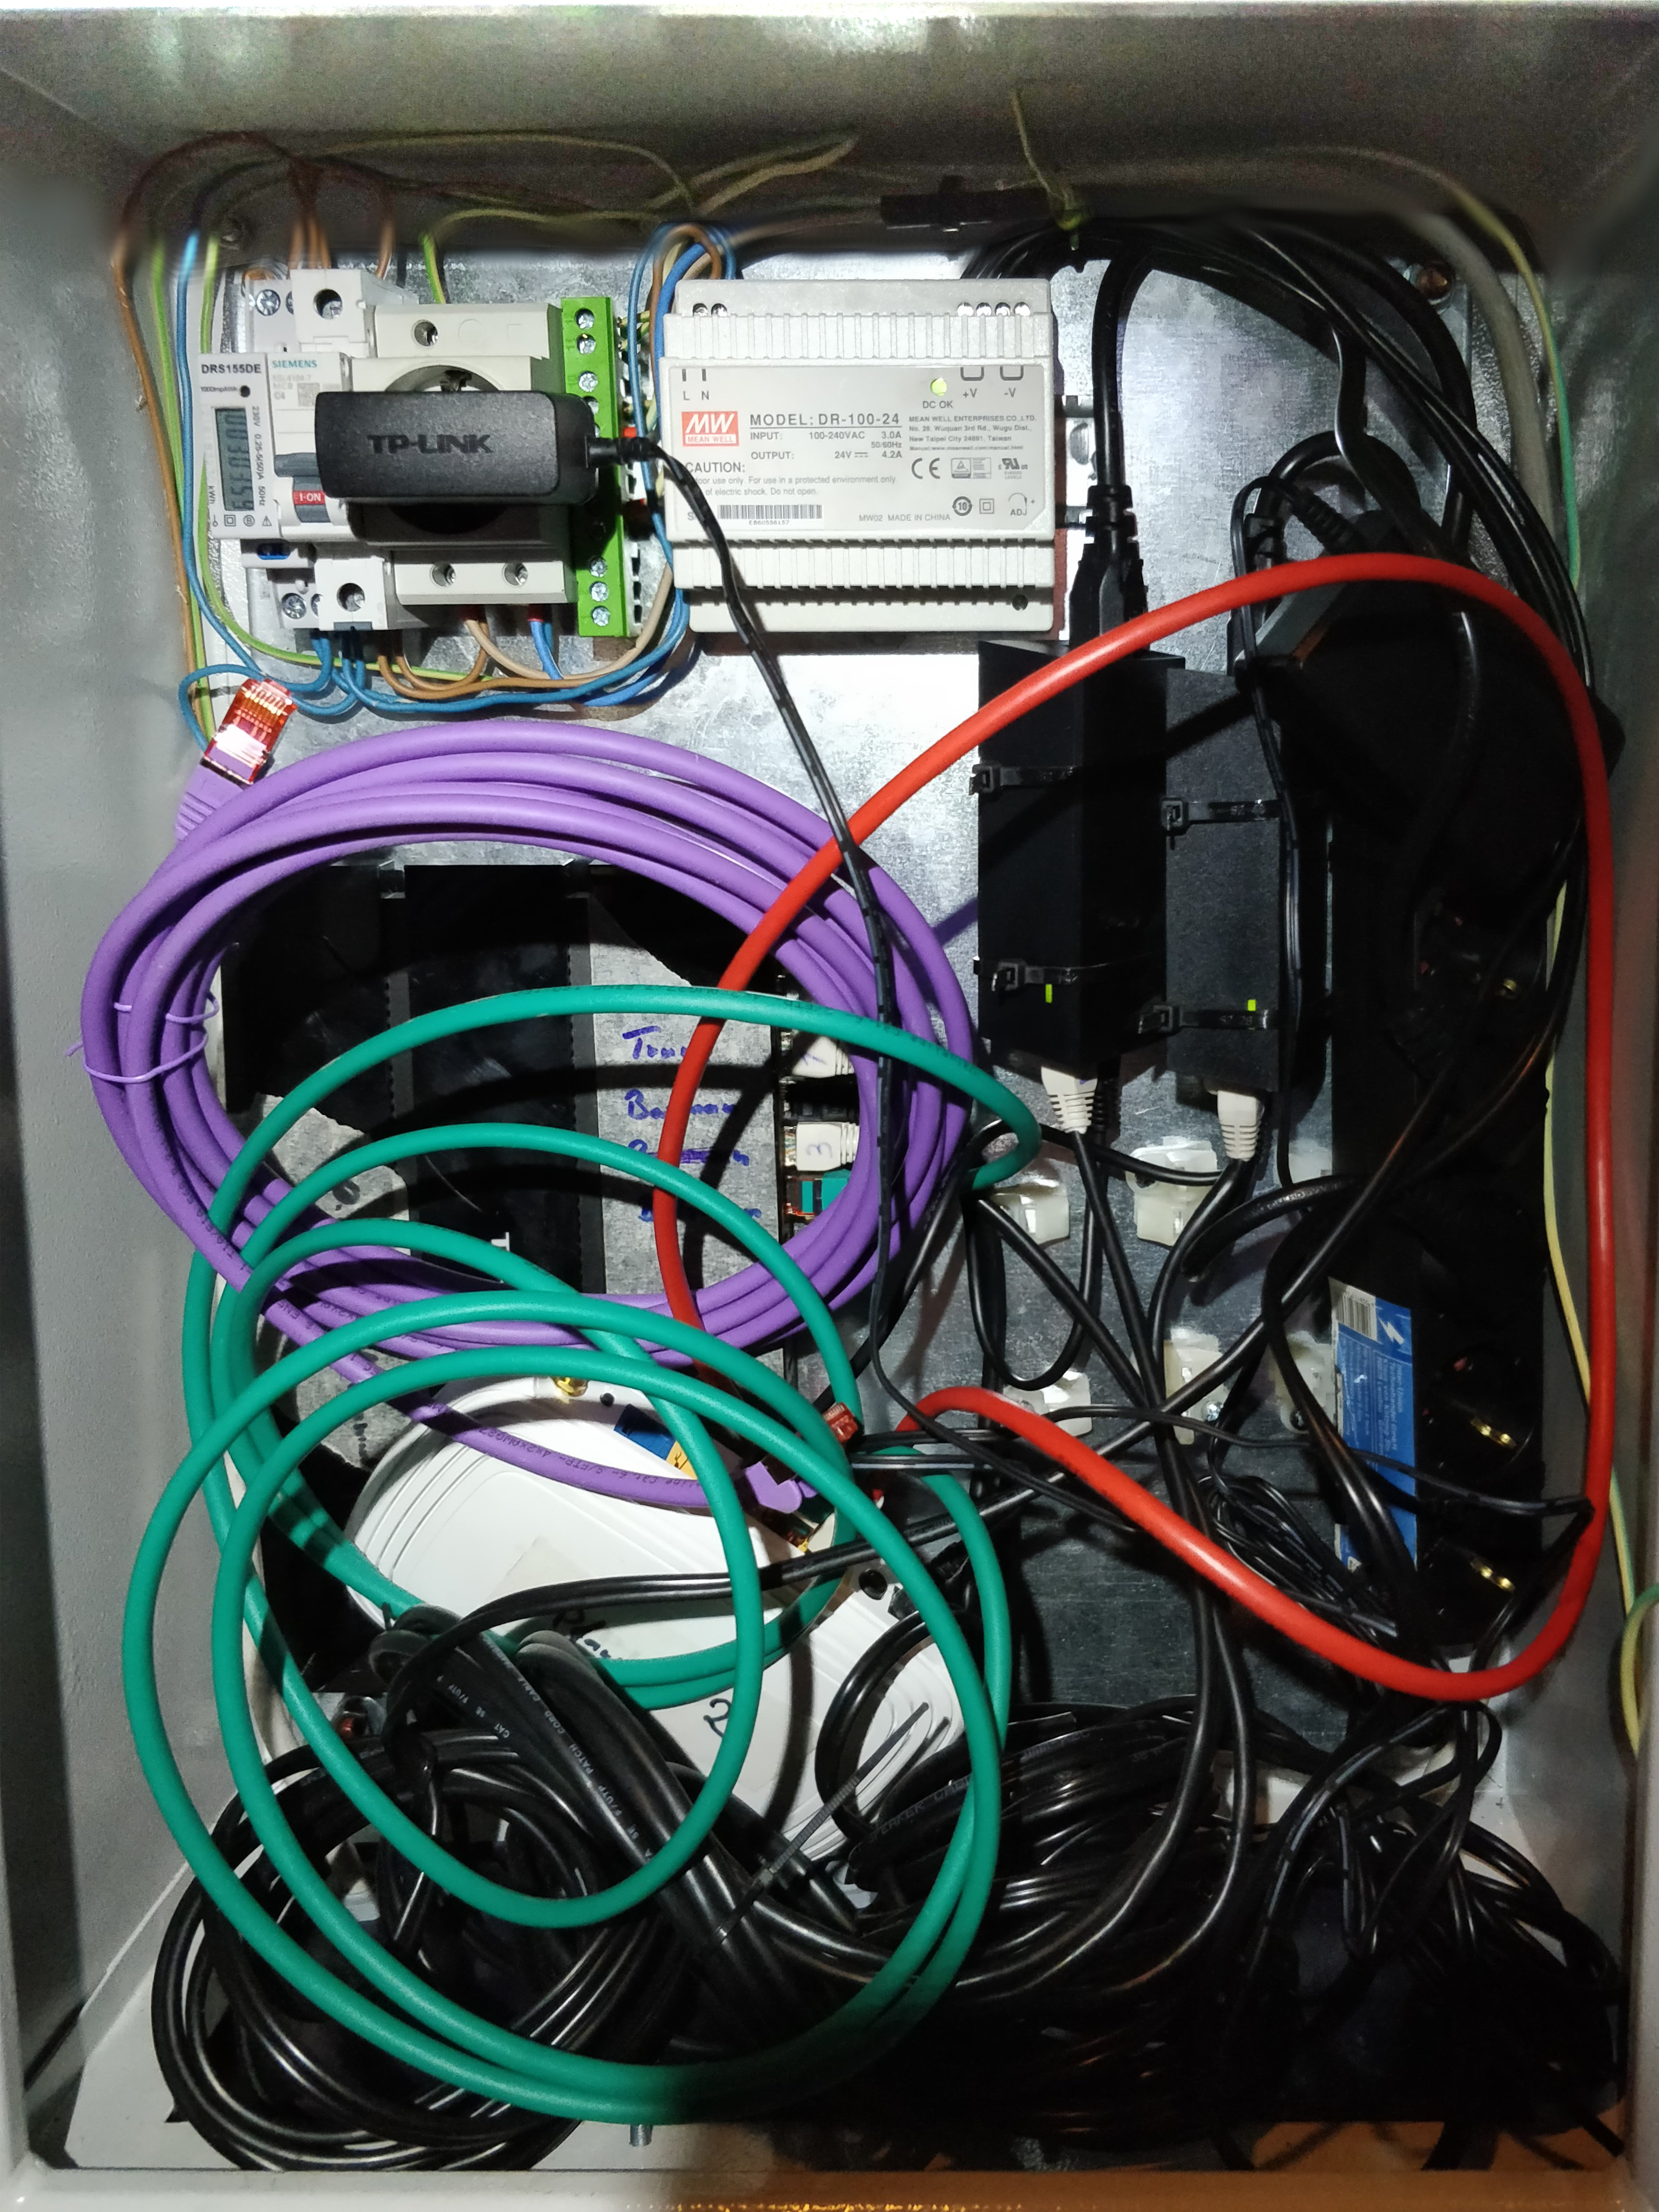
\includegraphics[height=0.86\textheight]{img/stpaul-kasten}
        \hfill
        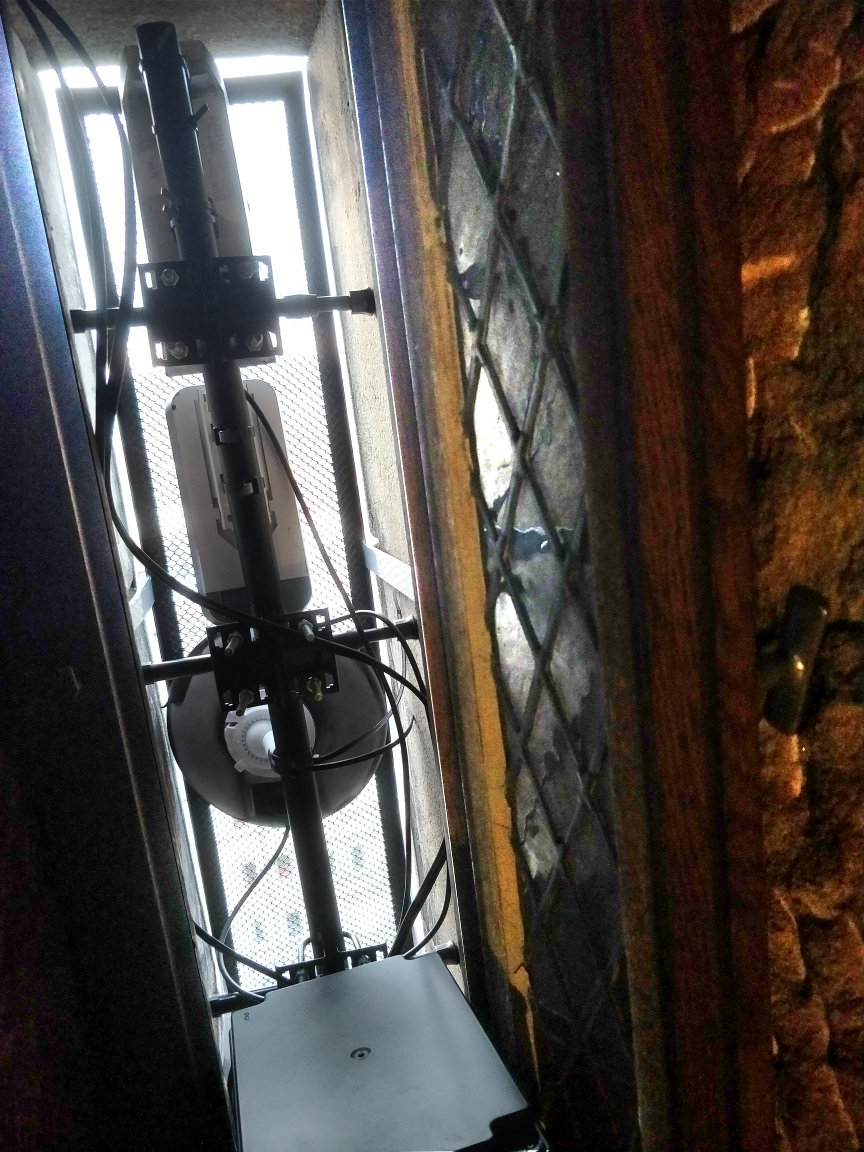
\includegraphics[height=0.86\textheight]{img/stpaul-fenster}
        \hfill
        ~
    }
\end{frame}

\section{Zusammenfassung}
\begin{frame}{}
    \begin{center}
        Zusammenfassung
     \end{center}
\end{frame}

\begin{frame}{Freifunk V1}
    \begin{itemize}
        \item Aktuelle (!) veraltete (!) Freifunk Firmware
        \begin{itemize}
            \item VPN Schlüsseltausch über zentrales Tool
            \item Manuelle Zuweisung der VPN Server
            \item Keine Anpassung an Firmware
            \item[$\rightarrow$] Loop durch versehentliches Meshing
        \end{itemize}
        \item Einseitiges Peering (viel Ausnutzung)
        \begin{itemize}
            \item[$\rightarrow$] Viele Router-Aufsteller
            \item[$\rightarrow$] Zu wenig Vernetzung
        \end{itemize}
    \end{itemize}
\end{frame}

\begin{frame}{Freifunk V2}
    \begin{itemize}
        \item Zukünftige (?) Freifunk Firmware
        \begin{itemize}
            \item VPN Schlüsseltausch über zentrales Tool
            \item Manuelle Zuweisung der VPN Server
            \item Theoretisch keine Loops
            \item[$\rightarrow$] Komplexität (viel) zu hoch
        \end{itemize}
        \item Einseitiges Peering (viel Ausnutzung)
        \begin{itemize}
            \item[$\rightarrow$] Viele Router-Aufsteller
            \item[$\rightarrow$] Zu wenig Vernetzung
        \end{itemize}
    \end{itemize}
\end{frame}

\begin{frame}{Freifunk V3}
    \begin{itemize}
        \item Zukünftige Freifunk Vernetzung
        \begin{itemize}
            \item Kein automatisches Peering
            \item[$\rightarrow$] Weniger Router-Aufstellern
        \end{itemize}
        \item Kaum Doku
        \item Manuelles Peering nötig
        \begin{itemize}
            \item Viel (soziale) Vernetzung
            \item Wecken von Potential
        \end{itemize}
        \item Layer 3 Routing
        \begin{itemize}
            \item Sehr hohe Performance
            \item Leichtes Debuggen
            \item Standard Komponenten
        \end{itemize}
    \end{itemize}
\end{frame}


\begin{frame}{Ende}
    \begin{center}
        Vielen Dank für eure Aufmerksamkeit!
     \end{center}
\end{frame}\addtocounter{framenumber}{-1}

\section*{}
\begin{frame}{Erinnerung: Gemeinnützigkeit}
    \begin{center}
        
\includegraphics[width=0.4\textwidth]{img/betterplace}\\\vspace{-0.2cm}
        \url{https://www.betterplace.org/de/projects/60168}
     \end{center}
\end{frame}\addtocounter{framenumber}{-1}
	
%%%%%%%%%%%%%%%%%%%%%% /CONTENT %%%%%%%%%%%%%%%%%%%%%%%%%%%%

\end{document}
